\documentclass{article}
\usepackage[tmargin=0.2in, lmargin=0.15in, rmargin=0.1in]{geometry}
\usepackage{fancyvrb}
\usepackage{floatrow}
\usepackage{graphicx}
\usepackage{amsmath}
\usepackage{caption}
\usepackage{subcaption}
\usepackage{pgfplots}
\title{\huge Run-and-tumble chemotaxis \\ \large Complete simulation for ML-agent and ideal agent}
\date{\today}
\begin{document}
\newcommand\nfig{1}
\newcommand\figext{.eps}
\maketitle

\noindent\hrulefill
\VerbatimInput{inputs.py}
\noindent\hrulefill


\vfill 
\noindent Parameters for manuscript Figure 1:
\VerbatimInput{data/sample_args.csv}
\pagebreak
\begin{minipage}{0.55\textwidth}
\begin{figure}[H]
\includegraphics[scale=1.0]{fig/conc_profile\figext}
\caption*{Concentration profile}
\end{figure}
\end{minipage}
\begin{minipage}{0.25\textwidth}
\VerbatimInput{data/conc_profile.txt}
\end{minipage}\hfill

\begin{minipage}{0.48\textwidth}
\begin{figure}[H]
\includegraphics[scale=1.0]{fig/init_position\figext}
\end{figure}
\end{minipage}
\begin{minipage}{0.48\textwidth}
\begin{figure}[H]
\includegraphics[scale=1.0]{fig/score\figext}
\caption*{Figure for SM}
\end{figure}
\end{minipage}\hfill

\begin{figure}[H]
\begin{center}
\hspace*{-1cm}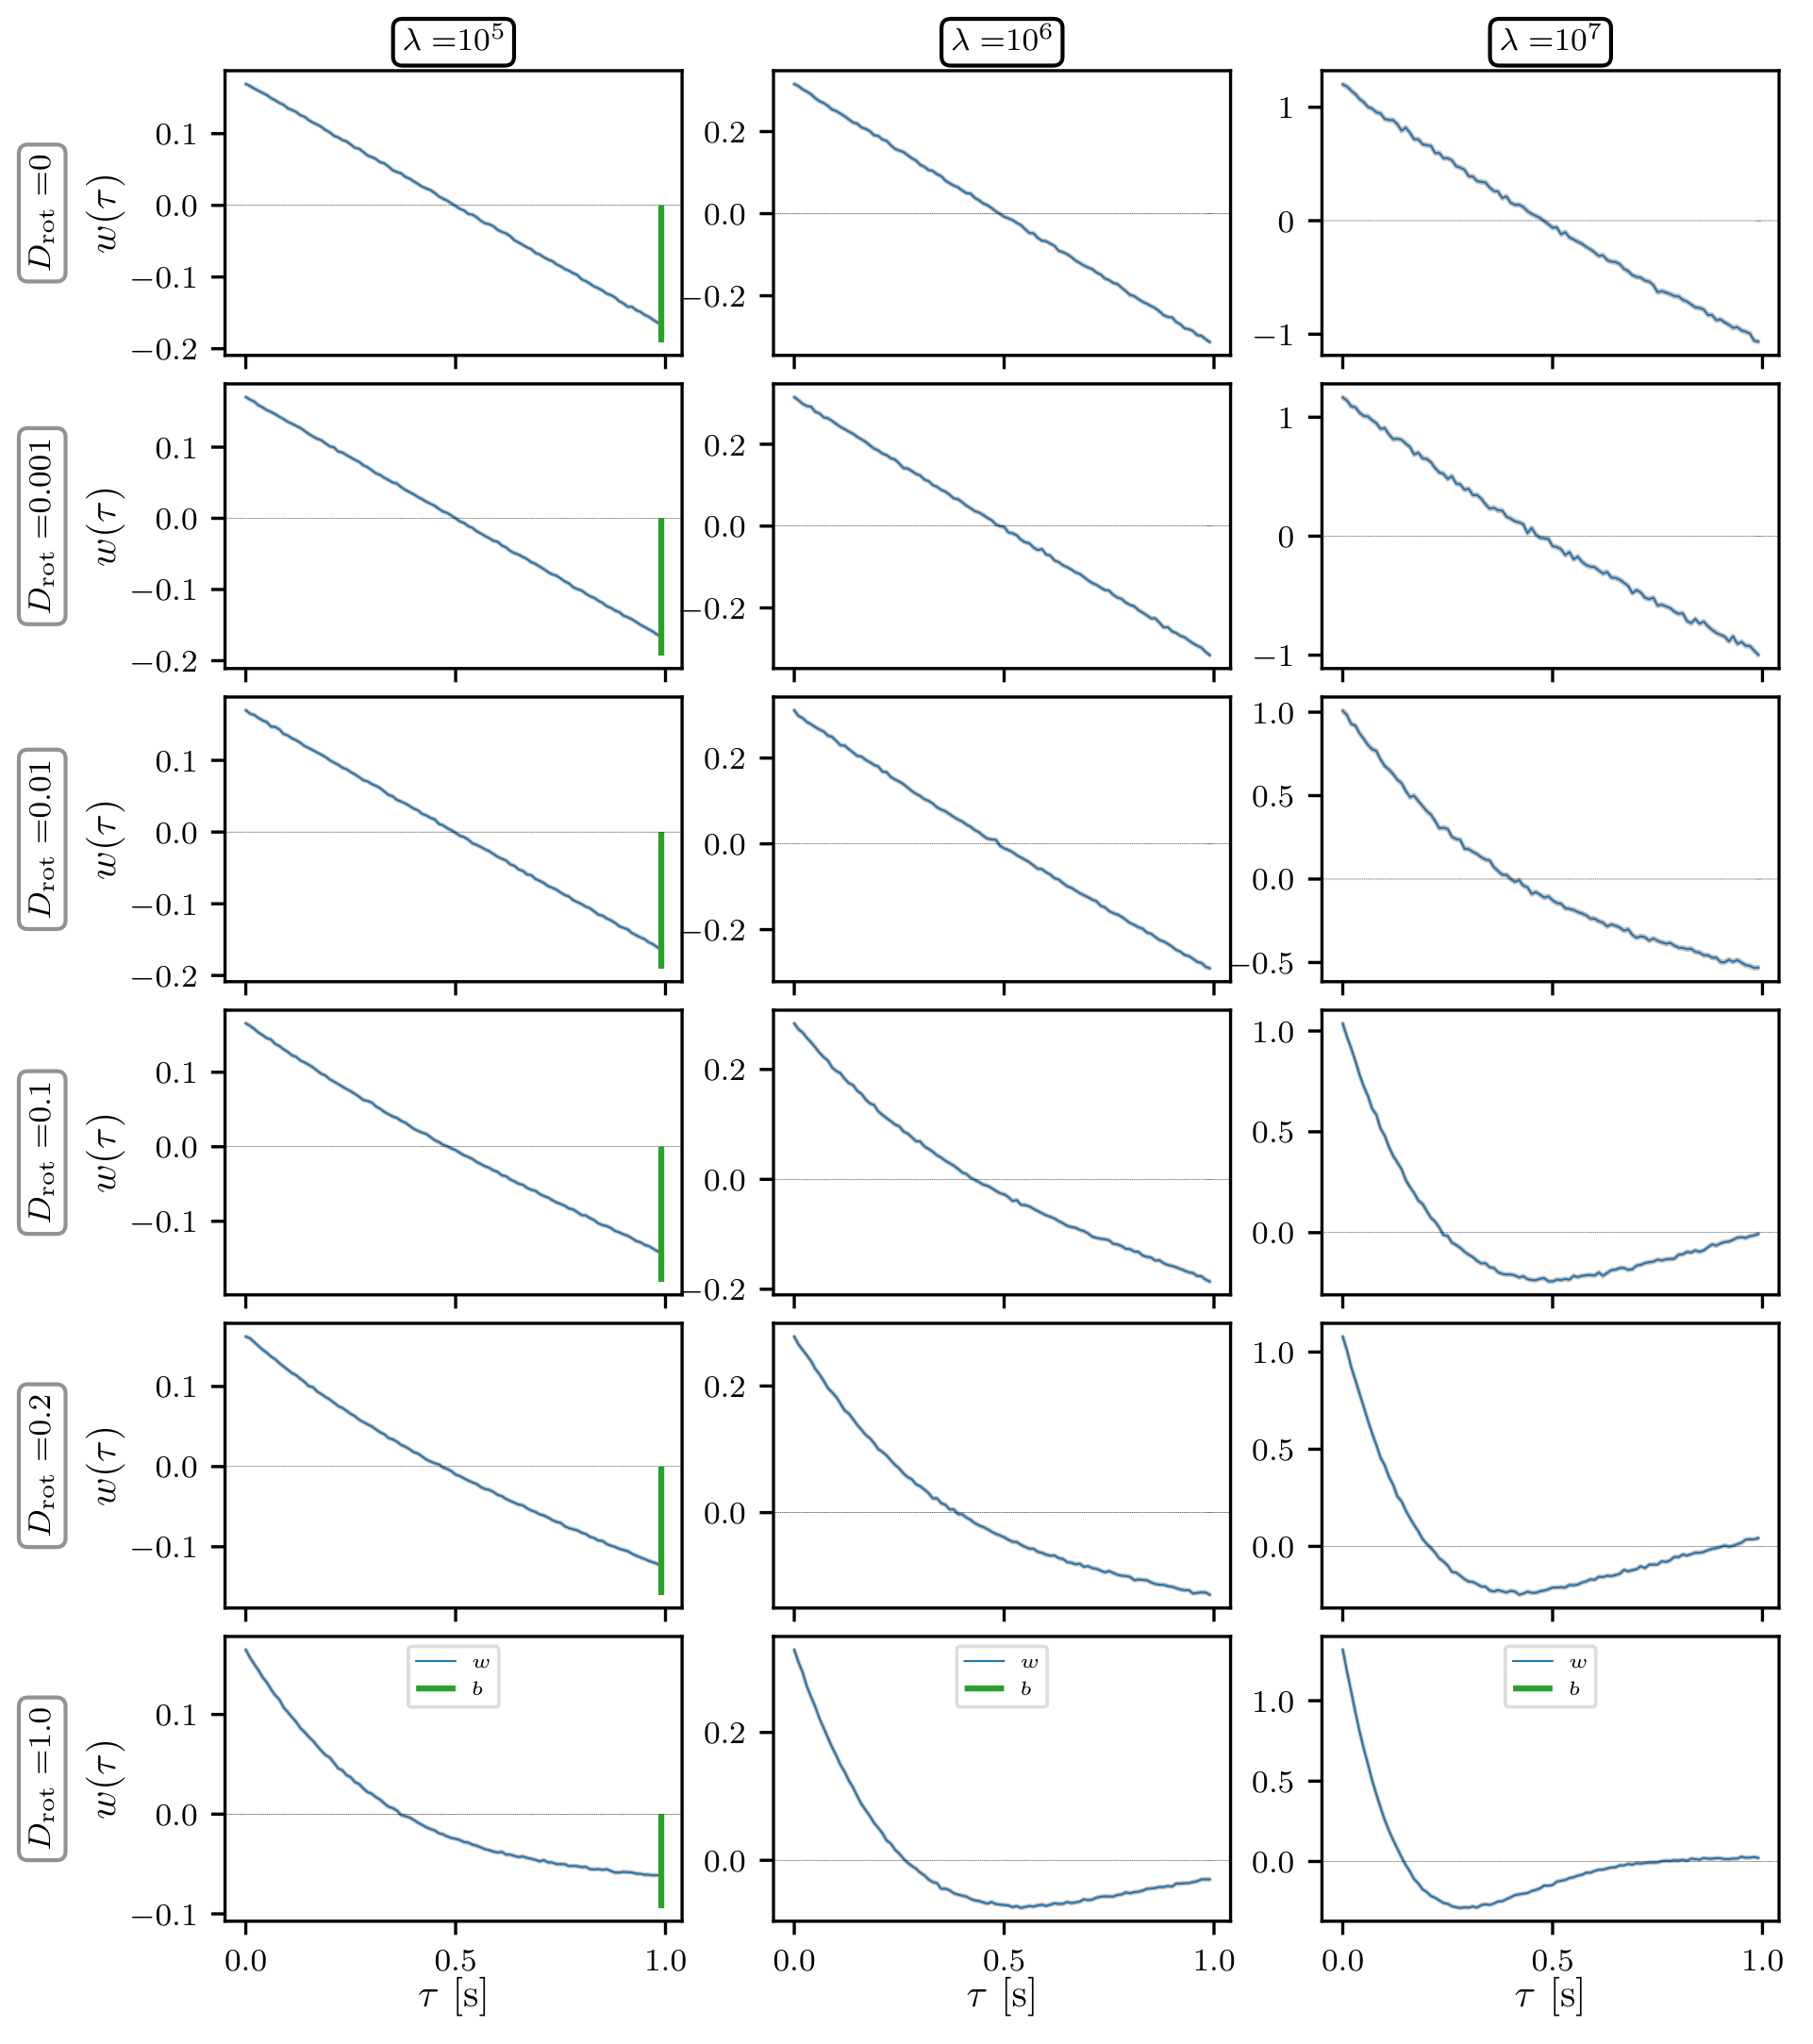
\includegraphics[scale=1.0]{fig/weights_grid.pdf}
\end{center}
\caption*{\textbf{weight profiles}: Figure for SM}
\end{figure}

\begin{figure}[H]
\begin{center}
\hspace*{-1cm}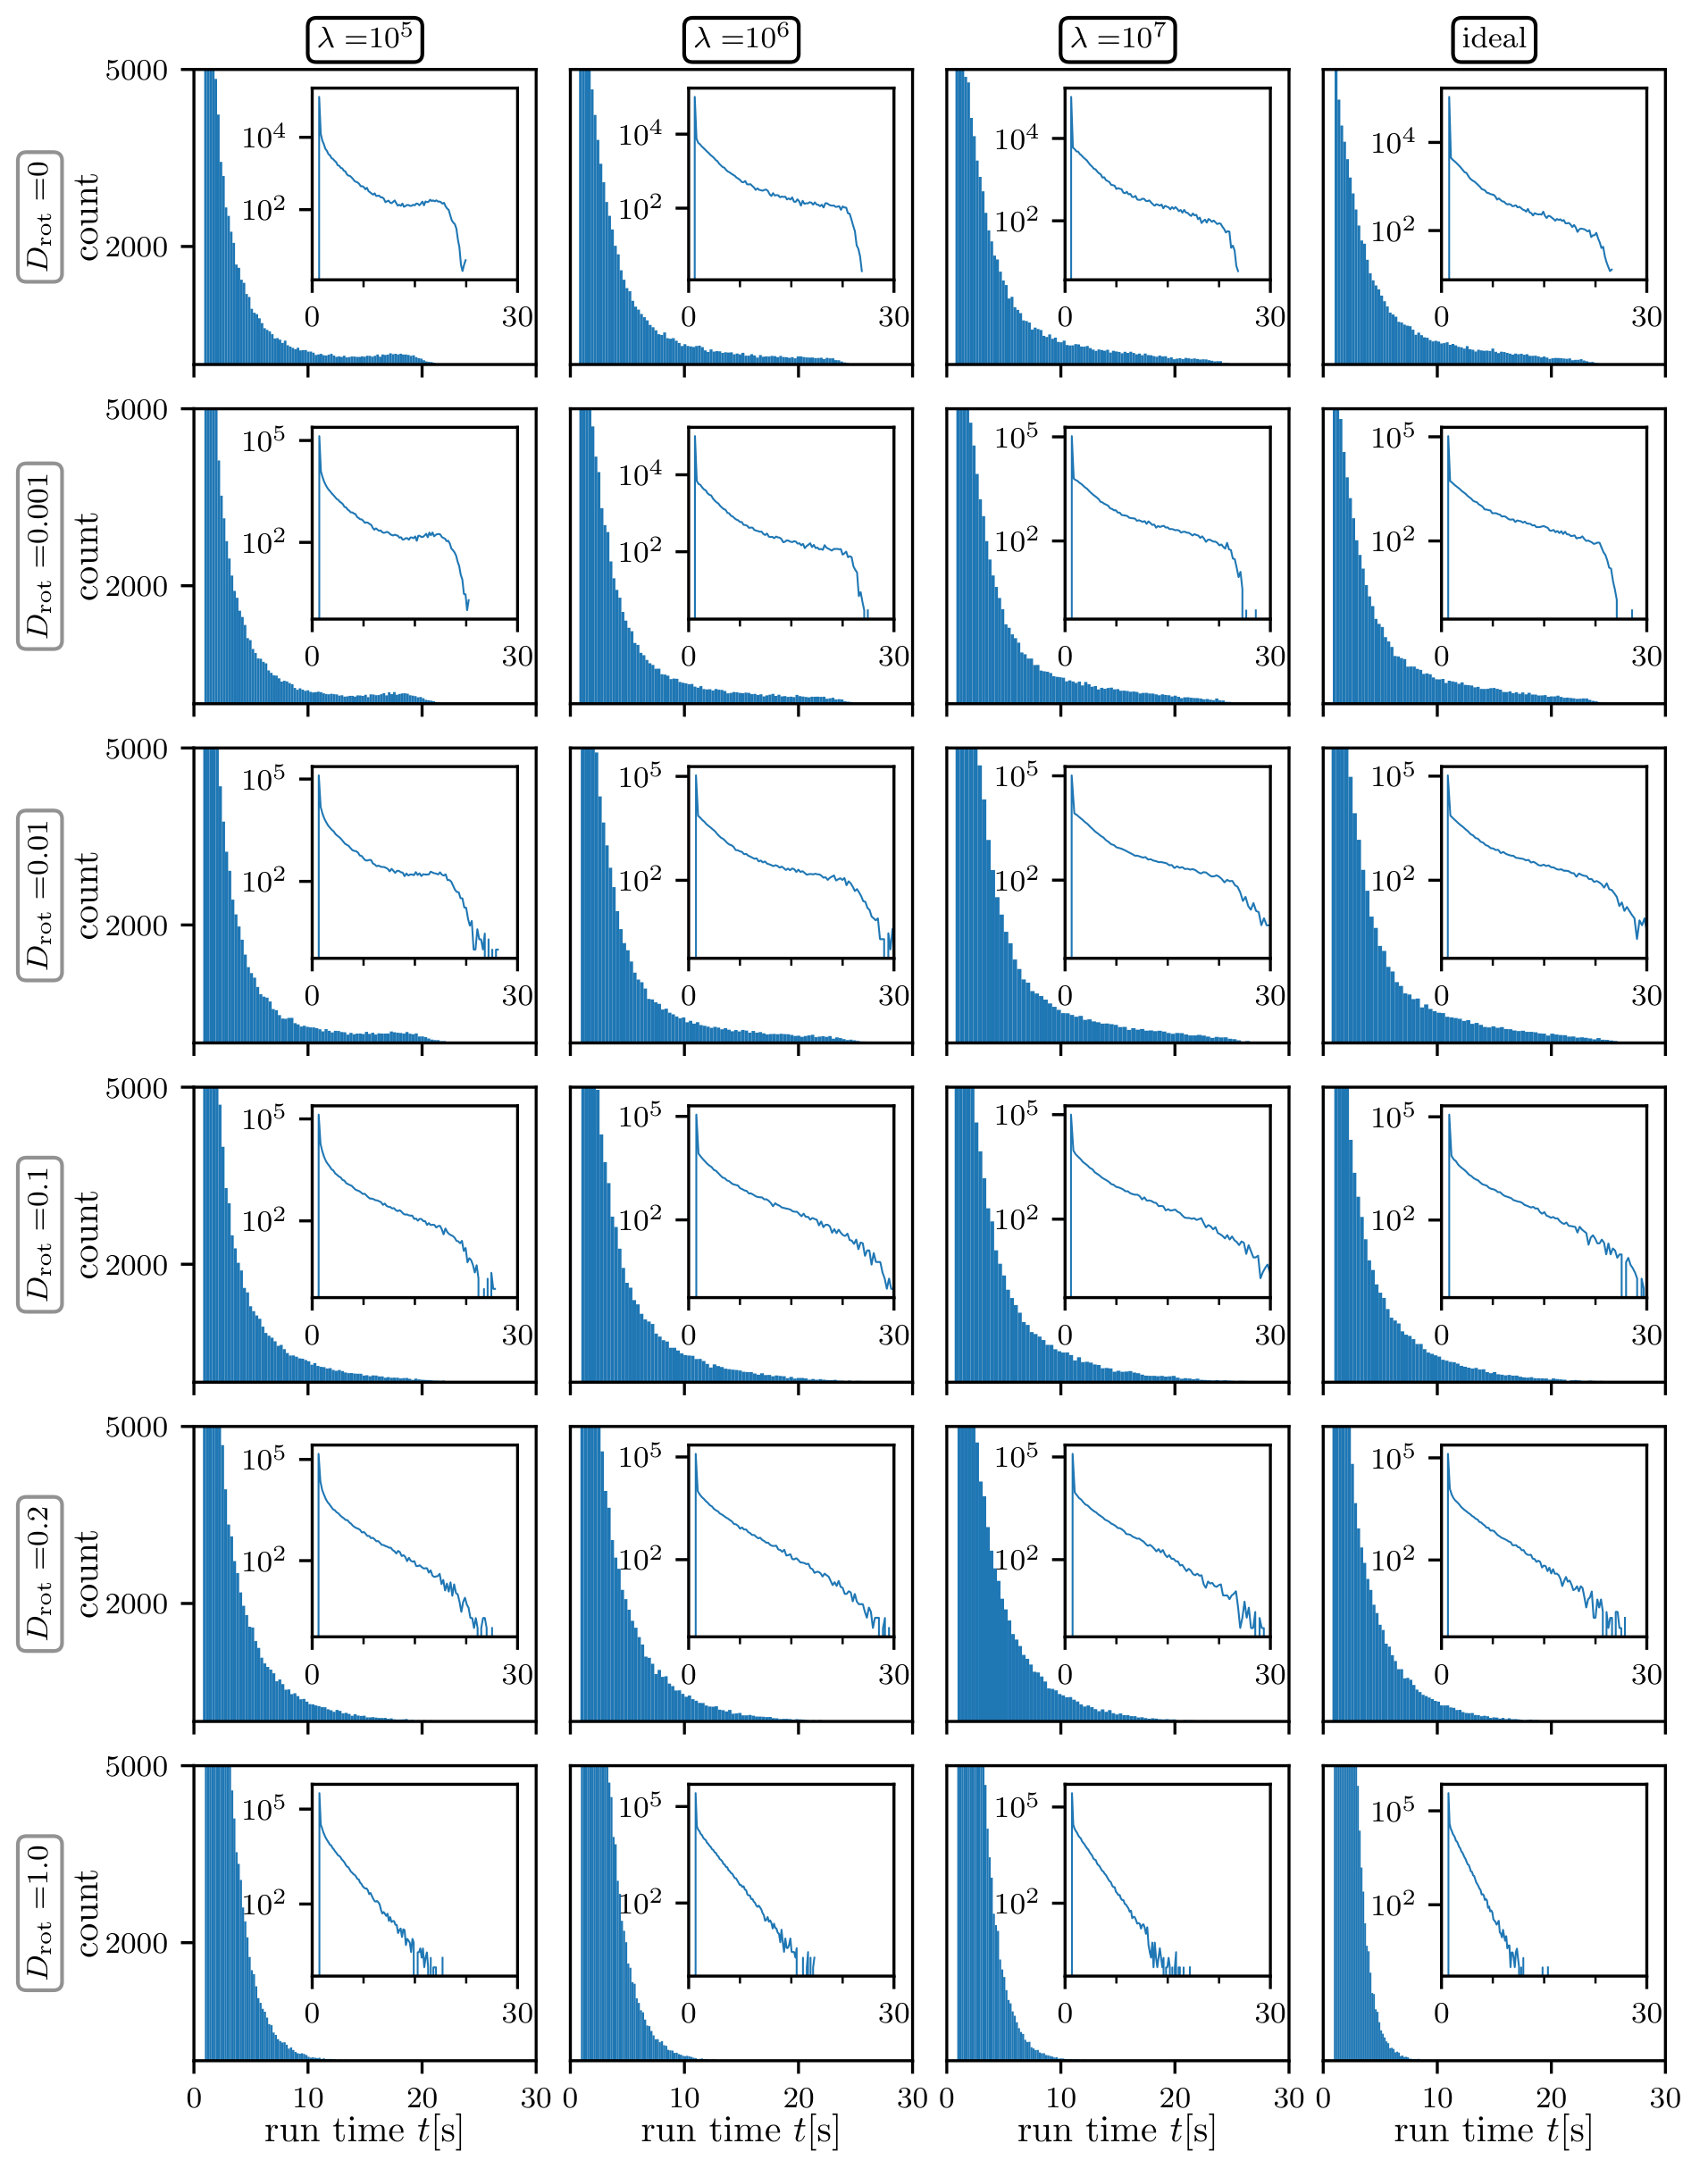
\includegraphics[scale=1.0]{fig/runtime_grid.pdf}
\end{center}
\caption*{\textbf{runtime}: Figure for SM}
\end{figure}

\pagebreak
\section*{Figures for the main text of the manuscript}

\begin{figure}[H]
\includegraphics[scale=1.0]{figure1\figext}
\caption*{Manuscript Figure 1}
\end{figure}



\begin{figure}[H]
\includegraphics[scale=1.0]{figure2\figext}
\caption*{Manuscript Figure 2}
\end{figure}

\begin{figure}[H]
\includegraphics[scale=1.0]{figure4\figext}
\caption*{Manuscript Figure 4}
\end{figure}

\thispagestyle{empty}
\end{document}



\begin{figure}[H]
\includegraphics[scale=1.0]{figure3\figext}
\end{figure}
